% Document Head
\documentclass[11pt, oneside]{book}
\usepackage{geometry}
\geometry{letterpaper}
\usepackage[parfill]{parskip}
\usepackage{graphicx}

% Essential Packages
\usepackage{ragged2e}
\usepackage{amssymb}
\usepackage{amsmath}
\usepackage{mathrsfs}
\usepackage[utf8]{inputenc}
\usepackage[english]{babel}
\usepackage{pgf,tikz}
\usepackage{pgfplots}
\usepackage[hyperref]{ntheorem}
\usepackage{hyperref}
\usepackage[noabbrev,capitalize,nameinlink]{cleveref}

% hyperref Package Settings
\usepackage{hyperref}
\hypersetup{
	colorlinks = true,
	linkcolor = magenta
}

% tikz Libraries
\usepgfplotslibrary{polar}
\usepgflibrary{shapes.geometric}
\usetikzlibrary{calc}

% Theorem Style Customization
\setlength\theorempreskipamount{2ex}
\setlength\theorempostskipamount{3ex}

% ntheorem Declarations
\theoremstyle{break}
\newtheorem{thm}{Theorem}[section]
\newtheorem*{proof}{Proof}
\newtheorem{crly}{Corollary}[section]
\newtheorem{lemma}{Lemma}[section]
\newtheorem{propo}{Proposition}[section]
\newtheorem*{remark}{Remark}
\newtheorem*{note}{Note}
\newtheorem*{notation}{Notation}
\newtheorem{ex}{Exercise}[section]
\newtheorem{defn}{Definition}[section]
\newtheorem{eg}{Example}[section]
\newtheorem{axiom}{Axiom}[section]

% ntheorem listtheorem style
\makeatother
\newlength\widesttheorem
\AtBeginDocument{
  \settowidth{\widesttheorem}{Proposition A.1.1.1\quad}
}

\makeatletter
\def\thm@@thmline@name#1#2#3#4{%
        \@dottedtocline{-2}{0em}{2.3em}%
                   {\makebox[\widesttheorem][l]{#1 \protect\numberline{#2}}#3}%
                   {#4}}
\@ifpackageloaded{hyperref}{
\def\thm@@thmline@name#1#2#3#4#5{%
    \ifx\#5\%
        \@dottedtocline{-2}{0em}{2.3em}%
            {\makebox[\widesttheorem][l]{#1 \protect\numberline{#2}}#3}%
            {#4}
    \else
        \ifHy@linktocpage\relax\relax
            \@dottedtocline{-2}{0em}{2.3em}%
                {\makebox[\widesttheorem][l]{#1 \protect\numberline{#2}}#3}%
                {\hyper@linkstart{link}{#5}{#4}\hyper@linkend}%
        \else
            \@dottedtocline{-2}{0em}{2.3em}%
                {\hyper@linkstart{link}{#5}%
                  {\makebox[\widesttheorem][l]{#1 \protect\numberline{#2}}#3}\hyper@linkend}%
                    {#4}%
        \fi
    \fi}
}

\makeatletter
\def\thm@@thmline@noname#1#2#3#4{%
        \@dottedtocline{-2}{0em}{5em}%
                   {{\protect\numberline{#2}}#3}%
                   {#4}}
\@ifpackageloaded{hyperref}{
\def\thm@@thmline@noname#1#2#3#4#5{%
    \ifx\#5\%
        \@dottedtocline{-2}{0em}{5em}%
            {{\protect\numberline{#2}}#3}%
            {#4}
    \else
        \ifHy@linktocpage\relax\relax
            \@dottedtocline{-2}{0em}{5em}%
                {{\protect\numberline{#2}}#3}%
                {\hyper@linkstart{link}{#5}{#4}\hyper@linkend}%
        \else
            \@dottedtocline{-2}{0em}{5em}%
                {\hyper@linkstart{link}{#5}%
                  {{\protect\numberline{#2}}#3}\hyper@linkend}%
                    {#4}%
        \fi
    \fi}
}

\theoremlisttype{allname}

% Custom math operator
% \DeclareMathOperator{\rem}{rem}
\DeclareMathOperator{\re}{Re}
\DeclareMathOperator{\im}{Im}

% Graph styles
\pgfplotsset{compat=1.15}
\usepgfplotslibrary{fillbetween}
\pgfplotsset{four quads/.append style={axis x line=middle, axis y line=
middle, xlabel={$x$}, ylabel={$y$}, axis equal }}
\pgfplotsset{four quad complex/.append style={axis x line=middle, axis y line=
middle, xlabel={$\re$}, ylabel={$\im$}, axis equal }}

% Shortcuts
\newcommand{\floor}[1]{\lfloor #1 \rfloor}      % simplifying the writing of a floor function
\newcommand{\ceiling}[1]{\lceil #1 \rceil}      % simplifying the writing of a ceiling function
\newcommand{\dotp}{\, \cdotp}			        % dot product to distinguish from \cdot
\newcommand{\qed}{\hfill\ensuremath{\square}}   % Q.E.D sign
\newcommand{\abs}[1]{\left|#1\right|}						% absolute value

% Main Body
\title{PMATH352W18 Complex Analysis - Class Notes}
\author{Johnson Ng}

\begin{document}
\hypersetup{pageanchor=false}
\maketitle
\hypersetup{pageanchor=true}
\tableofcontents

\chapter*{List of Definitions}
\theoremlisttype{all}
\listtheorems{defn}

\chapter*{List of Theorems}
\theoremlisttype{allname}
\listtheorems{axiom,lemma,thm,crly,propo}

\chapter{Lecture 1 - Jan 3, 2018}\label{chp:Lecture 1 - Jan 3, 2018}

\section{Complex Numbers and Their Properties}\label{sect:Complex Numbers and Their Properties}

\begin{defn}[Complex Number, Complex Plane]\label{defn:Complex Number, Complex Plane}
	A \textbf{complex number} is a vector in $\mathbb{R}^2$. The \textbf{complex plane}, denoted by $\mathbb{C}$, is a set of complex numbers,
	\begin{equation*}
		\mathbb{C} = \mathbb{R}^2 = \left\{ \begin{pmatrix} x \\ y \end{pmatrix} : x , y \in \mathbb{R} \right\}
	\end{equation*}
	In $\mathbb{C}$, we usually write \\
	\begin{center}
		\begin{tabular}{c c}
			$0 = \begin{pmatrix} 0 \\ 0 \end{pmatrix}$ & $1 = \begin{pmatrix} 1 \\ 0 \end{pmatrix}$ \\
			$i = \begin{pmatrix} 0 \\ 1 \end{pmatrix}$ & $x = \begin{pmatrix} x \\ 0 \end{pmatrix}$ \\
			$iy = \begin{pmatrix} 0 \\ y \end{pmatrix}$
		\end{tabular}
	\end{center}
	where $x, y \in \mathbb{R}$. Consequently, we have that
	\begin{equation*}
		x + iy = x + yi = \begin{pmatrix} x \\ y \end{pmatrix}
	\end{equation*}
	If for $x, y \in \mathbb{R}, \; z = x + iy$, then $x$ is aclled the real part of $z$ and $y$ is called the imaginary part of $z$, and we write
	\begin{equation*}
		\re(z) = x \quad \im(z) = y.
	\end{equation*}
\end{defn}

\begin{defn}[Sum and Product]\label{defn:Sum and Product}
	We define the sum of two complex numbers to be the usual vector sum, i.e.
	\begin{align*}
		(a + ib) + (c + id) &= \begin{pmatrix} a \\ b \end{pmatrix} + \begin{pmatrix} c \\ d \end{pmatrix} \\
											&= \begin{pmatrix} a + c \\ b + d \end{pmatrix} \\
											&= (a + c) + i (b + d)
	\end{align*}
	where $a, b, c, d \in \mathbb{R}$.

	We define the product of two complex numbers by setting $i^2 = -1$, and by requiring the product to be commutative, associative, and distributive over the sum. In this setup, we have that
	\begin{align}
		(a + ib)(c + id) &= ac + iad + ibc + i^2 bd \nonumber \\
						 &= (ac - bd) + i (ad + bc) \label{eq:complex multiplication}
	\end{align}
\end{defn}

\begin{eg}\label{eg:1}
	Let $z = 2 + i, w = 1 + 3i$. Find $z + w$ and $zw$.
	\begin{align*}
		z + w &= (2 + i) + (1 + 3i) \\
			  	&= 3 + 4i \\
			  	\\
		zw 		&= (2 + i)(1 + 3i) \\
					&= (2 - 3) + i (6 + 1) \quad \text{By } \cref{eq:complex multiplication}\\
					&= -1 + 7i
	\end{align*}
\end{eg}

\begin{eg}\label{eg:2}
	Show that every non-zero complex number has a multiplicative inverse, $z^{-1}$, and find a formula for this inverse.

	Let $z = a + ib$ where $a, b \in \mathbb{R}$ with $a^2 + b^2 \neq 0$. Then
	\begin{align*}
				 & z(x + iy) = 1 \\
		\iff & (ax - by) + i(ay + bx) = 1 \\
		\iff & \begin{pmatrix} ax - by \\ ay + bx	\end{pmatrix} = \begin{pmatrix} 1 \\ 0 \end{pmatrix} \\
		\iff & \begin{pmatrix} a & -b \\ b & a \end{pmatrix}\begin{pmatrix} x \\ y \end{pmatrix} = \begin{pmatrix} 1 \\ 0 \end{pmatrix} \\
		\iff & \begin{pmatrix} x \\ y \end{pmatrix} = \frac{1}{a^2 + b^2} \begin{pmatrix} a & b \\ -b & a \end{pmatrix}	\begin{pmatrix} 1 \\ 0 \end{pmatrix} \\
		\iff & \begin{pmatrix} x \\ y \end{pmatrix} = \frac{1}{a^2 + b^2}\begin{pmatrix} a \\ -b \end{pmatrix} \\
		\iff & x + iy = \frac{a}{a^2 + b^2} - i \frac{b}{a^2 + b^2} 
	\end{align*}
	Therefore, we have that the formula for the inverse is
	\begin{equation}\label{eq:complex inverse}
		(a + ib)^{-1} = \frac{a}{a^2 +b^2} - i \frac{b}{a^2 + b^2} 
	\end{equation}
\end{eg}

\begin{notation}
	For $z, w \in \mathbb{C}$, we write
	\begin{center}
		\begin{tabular}{c c}
			$-z = -1z$ & $w - z = w + (-z)$ \\
			$\frac{1}{z} = z^{-1}$ & $\frac{w}{z} = wz^{-1}$
		\end{tabular}
	\end{center}
\end{notation}

\begin{eg}\label{eg:3}
	Find $\frac{(4 - i) - (1 - 2i)}{1 + 2i}$.
	\begin{align*}
		\frac{(4 - i) - (1 - 2i)}{1 + 2i} &= \frac{3 + i}{1 + 2i} \\
					&= (3 + i)(\frac{1}{5} - i \frac{2}{5} ) \\
					&= 1 - i
	\end{align*}
\end{eg}

\begin{note}
	The set of complex numbers is a \textbf{field} under the operations of additiona and multiplication. This means that $\forall u, v, w \in \mathbb{C}$,
	\begin{center}
		\begin{tabular}{r@{\;{=}\;}l r@{\;{=}\;}l}
			u + v 			& v + u 			& uv 			& vu \\
			(u + v) + w & u + (v + w) & (uv)w 	& u(vw) \\
			0 + u 			& u 					& 1u			& u \\
			u + (-u)		& 0						& $uu^{-1}$	& 1, $\; u \neq 0$ \\
			u(v + w)		& uv + uw
		\end{tabular}
	\end{center}
\end{note}

\begin{defn}[Conjugate]\label{defn:Conjugate}
	If $z = x + iy$ where $x, y \in \mathbb{R}$, then the $\textbf{conjugate of z}$ is given by $\bar{z} = x - iy$
\end{defn}

\begin{eg}\label{eg:4}
	Let $z = 3 + 4i$. Then the $\bar{z} = 3 - 4i$. Represented in the complex plane, we have the following:
	\begin{center}
		\begin{tikzpicture}
			\begin{axis}[four quad complex, xtick={-4,-3,...,4}, ytick={-5,-4,...,5}, xmin=-4, xmax=4, ymin=-5, ymax=5]
				\node[label={0:{$z$}},circle,fill,inner sep=2pt] at (axis cs:3,4) {};
				\node[label={0:{$\bar{z}$}},circle,fill,inner sep=2pt] at (axis cs:3,-4) {};
			\end{axis}
		\end{tikzpicture}
	\end{center}
\end{eg}

\begin{defn}[Modulus]\label{defn:Modulus}
	We define the \textbf{modulus} (length, magnitude) of $z = x + iy \in \mathbb{C}, x, y \in \mathbb{R}$, to be
	\begin{equation}
		\abs{z} = \sqrt{x^2 + y^2} \in \mathbb{R}.
	\end{equation}
\end{defn}

\begin{note}
 For $z, w \in \mathbb{R}$, we have
 \begin{center}
 	\begin{tabular}{r@{\;{=}\;}l r@{\;{=}\;}l r@{\;{=}\;}l}
 		$\bar{\bar{z}}$ 	& z 									& $z + \bar{z}$ 	& $2 \re(z)$ 			& $z - \bar{z}$ 	& $2i \im(z)$ \\
 		$z\bar{z}$				& $\abs{z}^2$					& $\abs{z}$				& $\abs{\bar{z}}$	& $\overline{z \pm w}$	& $\bar{z} \pm \bar{w}$ \\
 		$\overline{zw}$		& $\bar{z} - \bar{w}$	& $\abs{zw}$			&	$\abs{z}\abs{w}$
 	\end{tabular}
 \end{center}
 but note that $\abs{z + w} \neq \abs{z} + \abs{w}$.
\end{note}

\begin{propo}[Basic Inequalities]\label{propo:Basic Inequalities}
	\begin{enumerate}
		\item $\abs{\re(z)} \leq \abs{z}$ \\
		\item $\abs{\im(z)} \leq \abs{z}$ \\
		\item $\abs{z + w} \leq \abs{z} + \abs{w} \quad$ Triangle Inequality \\
		\item $\abs{z + w} \geq \abs{\;\abs{z} - \abs{w}\;} \quad$ Inverse Triangle Inequality
	\end{enumerate}
\end{propo}

\begin{proof}
	Note that $\abs{z}^2 = \re(z)^2 + \im(z)^2$ and that we can express $\abs{x} = \sqrt{x^2}$ for any $x \in \mathbb{R} $. 1 and 2 immediately follows from that.

	To prove 3, we have that
	\begin{align*}
		\abs{z + w}^2 &= (z + w)(\bar{z} + \bar{w}) \\
									&= \abs{z}^2 + \abs{w}^2 + (w\bar{z} + \bar{w}z) \\
									&= \abs{z}^2 + \abs{w}^2 + 2\re(w\bar{z}) \\
									&\leq \abs{z}^2 + \abs{w}^2 + 2\abs{w\bar{z}} \quad \text{by 1} \\
									&= \abs{z}^2 + \abs{w}^2 + 2\abs{wz} \quad \text{since } \abs{w\bar{z}} = \abs{w}\abs{\bar{z}} \text{ and } \abs{z} = \abs{\bar{z}} \\
									&= (\abs{z} + \abs{w})^2
	\end{align*}
	
	To prove 4, note that
	\begin{alignat}{3}
		&\abs{z} &&= \abs{z + w - w} &&\leq \abs{z + w} + \abs{w} \label{basicinequal1} \\
		&\abs{w} &&= \abs{w + z - z} &&\leq \abs{z + w} + \abs{z} \label{basicinequal2}
	\end{alignat}

	Observe that
	\begin{align*}
		\cref{basicinequal1} \implies \abs{z} - \abs{w} \leq \abs{z + w} \\
		\cref{basicinequal2} \implies \abs{w} - \abs{z} \leq \abs{z + w}
	\end{align*}

	Thus, we have that
	\begin{equation*}
		\abs{z + w} \geq \abs{\; \abs{z} - \abs{w} \;}
	\end{equation*}
	as required.\qed
\end{proof}

\begin{eg}
	We may describe a set $\left\{z \in \mathbb{C} : \abs{z -i} = 1 \right\}$ as follows:

	\begin{center}
		\begin{tikzpicture}
			\begin{axis}[four quad complex, xtick={-3,-2,...,3}, ytick={-3,-2,...,3}, xmin=-3, xmax=3, ymin=-1, ymax=3]
				\draw (axis cs:0, 1) circle [radius=1];
			\end{axis}
		\end{tikzpicture}
	\end{center}

	Let $a, b \in \mathbb{C}$ describe the set $\left\{z \in \mathbb{C} : \abs{z - a} < \abs{z - b} \right\}$.

	Suppose the following coordinates for $a$ and $b$ are arbitrary,

	\begin{center}
		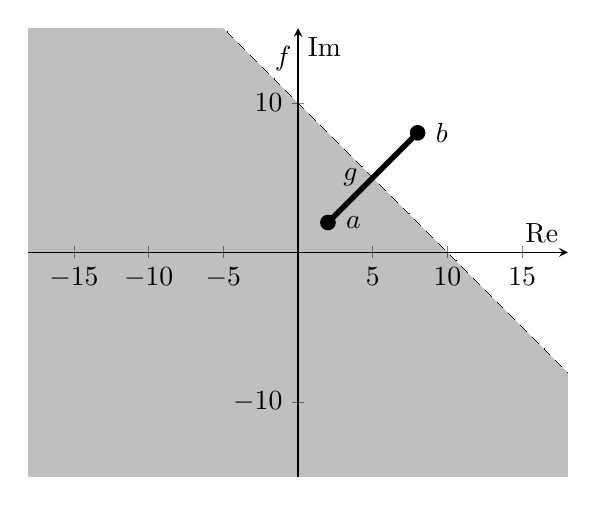
\begin{tikzpicture}
			\begin{axis}[four quad complex, xmin=-15, xmax=15, ymin=-15, ymax=15]
				\draw[line width=0pt,dashed,fill=black,fill opacity=0.25](-20,20)--(-20,-20)--(20,-20)--(20,-10)--(-5,15);
				\draw[color=black] (-1,13) node {$f$};
				\draw[line width=2pt,solid](2,2)--(8,8);
				\draw[color=black] (3.5,5) node {$g$};
				\node[label={0:{$a$}},circle,fill,inner sep=2pt] at (axis cs:2,2) {};
				\node[label={0:{$b$}},circle,fill,inner sep=2pt] at (axis cs:8,8) {};
			\end{axis}
		\end{tikzpicture}
	\end{center}

	In the above, $g$ is the line segment that connects the points $a$ and $b$ on the complex plane, while $f$ is the perpendicular bisector of the line segment $g$. The area described by the set $\left\{z \in \mathbb{C} : \abs{z - a} < \abs{z - b} \right\}$ is the shaded area which is below $f$.
\end{eg}

\begin{eg}
	Let $a \in \mathbb{C}$. Describe the set $\{z \in \mathbb{C} : 1 < \abs{z-a} < 2\}$.

	\begin{center}
		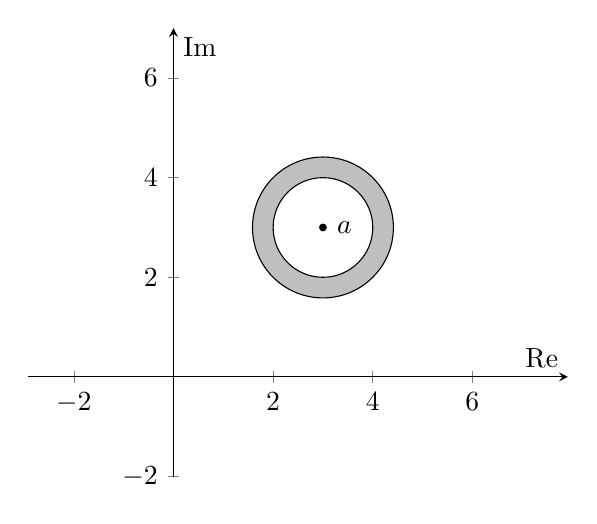
\begin{tikzpicture}
			\begin{axis}[
				four quad complex,
				xmin=-2, xmax=7,
				ymin=-2, ymax=7
			]
				\draw [fill=black,fill opacity=0.25] (3,3) circle (1.4142135623730951);
				\draw[fill=white](3,3) circle (1);
				\node[label={0:{$a$}},circle,fill,inner sep=1pt] at (axis cs:3,3) {};
			\end{axis}
		\end{tikzpicture}
	\end{center}
\end{eg}

\begin{eg}
	\label{eg:complex number has exactly two roots}
	Show that every non-zero complex number has exactly two complex square roots, and find a formula for the square roots.

	Let $z = x + iy \in \mathbb{C}, x, y \in \mathbb{R}$, and let $w = u + iv, u, v \in \mathbb{R}$. Then

	\begin{alignat}{3}
		&w^2 = z &&\iff && (u + iv)^2 = x + iy \nonumber \\
		&	&&\iff 	&& (u^2 - v^2) + i(2uv) = x + iy \nonumber \\
		&	&&\iff && x = u^2 + v^2 \quad \text{and} \label{tworoots 1} \\
		&	&&	   && y = 2uv \label{tworoots 2}
	\end{alignat}

	Square both sides of \cref{tworoots 2}, and thus we have $y^2 = 4u^2 v^2$.

	Multiply \cref{tworoots 1} by $4u^2$, and we get
	\begin{alignat*}{3}
		& 	  &&4u^2 x &&= 4u^4 - 4u^2 v^2 = 4u^4 - y^2 \\
		&\iff &&0 	&&= 4u^4 - 4u^2 x - y^2 \\
		&\iff &&u^2 &&= \frac{4x \pm \sqrt{16x^2 + 16y^2}}{8} \\
		&	  &&	&&= \frac{x \pm \sqrt{x^2 + y^2}}{2} 
	\end{alignat*}

	Suppose $y \neq 0$. Note that $x < \sqrt{x^2 + y^2}$. Thus $u^2 = \frac{x + \sqrt{x^2 + y^2}}{2} \implies u = \left(\frac{x + \sqrt{x^2 + y^2}}{2} \right)^{\frac{1}{2}}$.

	Similarly, we can get
	\begin{equation*}
		v = \pm \left(\frac{-x + \sqrt{x^2 + y^2}}{2}\right)^{\frac{1}{2}}
	\end{equation*}

	Note that all four choices of signs satisfy \cref{tworoots 1}. If $y > 0$, then $u$ and $v$ are either both positive or both negative by \cref{tworoots 2}.

	Suppose $y = 0$. Then we have
	\begin{equation*}
		w^2 = z = x
	\end{equation*}

	Therefore, we get
	\begin{equation*}
		w = \begin{cases}
			\pm \left[ \left(\frac{x + \sqrt{x^2 + y^2}}{2} \right)^{\frac{1}{2}} + i \left( \frac{-x + \sqrt{x^2 + y^2}}{2} \right)^{\frac{1}{2}} \right] & y > 0 \\
			\pm \left[ \left(\frac{x + \sqrt{x^2 + y^2}}{2} \right)^{\frac{1}{2}} - i \left(\frac{-x + \sqrt{x^2 + y^2}}{2} \right)^{\frac{1}{2}} \right] & y < 0 \\
			\pm \sqrt{x} & y = 0, x > 0 \\
			\pm i \sqrt{x} & y = 0, x < 0
		\end{cases}
	\end{equation*}
\end{eg}

\begin{remark}
	Let $z \in \mathbb{C}$. The notation $\sqrt{z}$ may represent either one of the square roots of $z$ or both of the square roots, i.e. it is possible that $\sqrt{z}$ represents a set.
\end{remark}

\begin{ex}\label{ex:Separation of Multiplication in Square Roots}
	Is it always okay for complex numbers such that $\sqrt{zw} = \sqrt{z} \sqrt{w}$, for $z, w \in \mathbb{C}$?

	No. For example, consider $z = w = -1$. Then we have
	\begin{equation*}
		\sqrt{zw} = \sqrt{1} = \pm 1
	\end{equation*}
	while
	\begin{equation*}
		\sqrt{z} \sqrt{w} = i \cdot i = -1
	\end{equation*}
	and thus
	\begin{equation*}
		\sqrt{zw} \neq \sqrt{z} \sqrt{w}.
	\end{equation*}
\end{ex}

\begin{eg}
	Find the values of $\sqrt{3 - 4i}$.

	By \cref{eg:complex number has exactly two roots},

	\begin{align*}
		\sqrt{3 - 4i} &= \pm \left( \sqrt{\frac{3 + \sqrt{9 + 16}}{2}} - i \sqrt{\frac{-3 + \sqrt{9 + 16}}{2}} \right) \\
			&= \pm (2 - i)
	\end{align*}
\end{eg}

\begin{remark}\label{remark:quadratic formula for complex numbers}
	The quadratic formula holds for complex polynomials, i.e.
	\begin{equation*}
		\forall a, b, c \in \mathbb{C} \quad a \neq 0 \quad \forall z \in \mathbb{C} \; az^2 + bz + c = 0,
	\end{equation*}
	the solution for $z$ is given by
	\begin{equation}\label{eq:quadractic formula for complex numbers}
		z_{1, 2} = \frac{-b + \sqrt{b^2 - 4ac}}{b} 
	\end{equation}

	The following is a short proof.

	\begin{proof}
		\begin{align*}
			az^2 + bz + c = 0 &\iff z^2 + \frac{b}{a} z + \frac{c}{a} = 0 \\
				&\iff z^2 + \frac{b}{a} z + \left(\frac{b}{2a} \right)^2 - \left(\frac{b}{2a}\right)^2 + \frac{c}{a} = 0 \\
				&\iff \left(z + \frac{b}{2a} \right)^2 = \frac{b^2}{4a^2} - \frac{c}{a} = \frac{b^2 - 4ac}{4a^2} \\
				&\iff z = \frac{-b + \sqrt{b^2 - 4ac}}{2a}  
		\end{align*}
	\end{proof}

	(Personal Note: where did the $-$ for the supposed $\pm$ go? Or should it really be $\pm$?)
\end{remark}

\begin{eg}
	Solve $iz^2 - (2 + 3i)z + 5(1 - i) = 0$.

	\begin{align*}
		z &= \frac{2 + 3i + \sqrt{(2 + 3i)^2 - 4i[5(1 - i)]}}{2i} \\
			&= \frac{2 + 3i + \sqrt{-5 + 12i - 20i - 20}}{2i} \\
			&= \frac{2 + 3i + \sqrt{-25 - 8i}}{2i} 
	\end{align*}

	\begin{align*}
		\sqrt{-25 - 8i} &= \pm \left[ \left(\frac{-25 + \sqrt{625 + 64}}{2} \right)^{\frac{1}{2}}  - i \left(\frac{25 + \sqrt{625 + 64}}{2} \right)^{\frac{1}{2}} \right]
	\end{align*}

	(Personal note: temporarily stuck, seeing that there's no ``nice'' solution)
\end{eg}

\end{document}